\section{Brake Test}\label{sec:brakeTest}

	\subsection{Full Stop Test}

		The desired test will be the full stop test, described by \cite{caixeta2017} as a test where the speed is set to a upper limit and then to nought rotation at the end. In order to achieve more reliable data the test shall be carried a hundred times.

		\par
		In order to start the brake test the following parameters were configured on the \textit{Labview} Test Application:

		\begin{itemize}
			\item\textit{Number of Snubs:} In order to achieve solid results, 100 snubs were set.
			\item\textit{Interval between snubs (s):} In order to let the brake pads cool, five seconds were set between each snub.
			\item\textit{Upper Limit (RPM):} The upper limit was set at 500 RPMs, that is almost the fastest measured rotation that the brake machine can achieve.
			\item\textit{Upper Wait Interval (s):} Three seconds, just enough so that the speed can stabilize.
			\item\textit{Lower Limit (RPM):} Nought, the idea is to fully stop the system.
			\item\textit{Lower Wait Interval (s):} Nought, as the \textit{Lower Limit (RPM)} will be zero, this time can be compreheended inside the \textit{Inverval Between Snubs}.
		\end{itemize}

		The goal of this tests is not to evaluate braking performance of components of a brake system but rather to prove that the developed hardware can be used for that, i.e. showing that the measured quantities are directly related to the tests are being carried out. Hence, temperature should increase after each snub, the measured braking pressure should increase and the CKP signal frequency should decrease rapidly as the braking actuator is activated. Moreover, it shall be possible to see a variation in brake efficiency when the brakes are hotter.

	\subsection{Results and Discussion}

		Figure \ref{fig:test-first-ten-snubs} shows a graph with the measured quantities on the first ten of the hundred snubs.

		\begin{figure}[htbp]
				\centering
				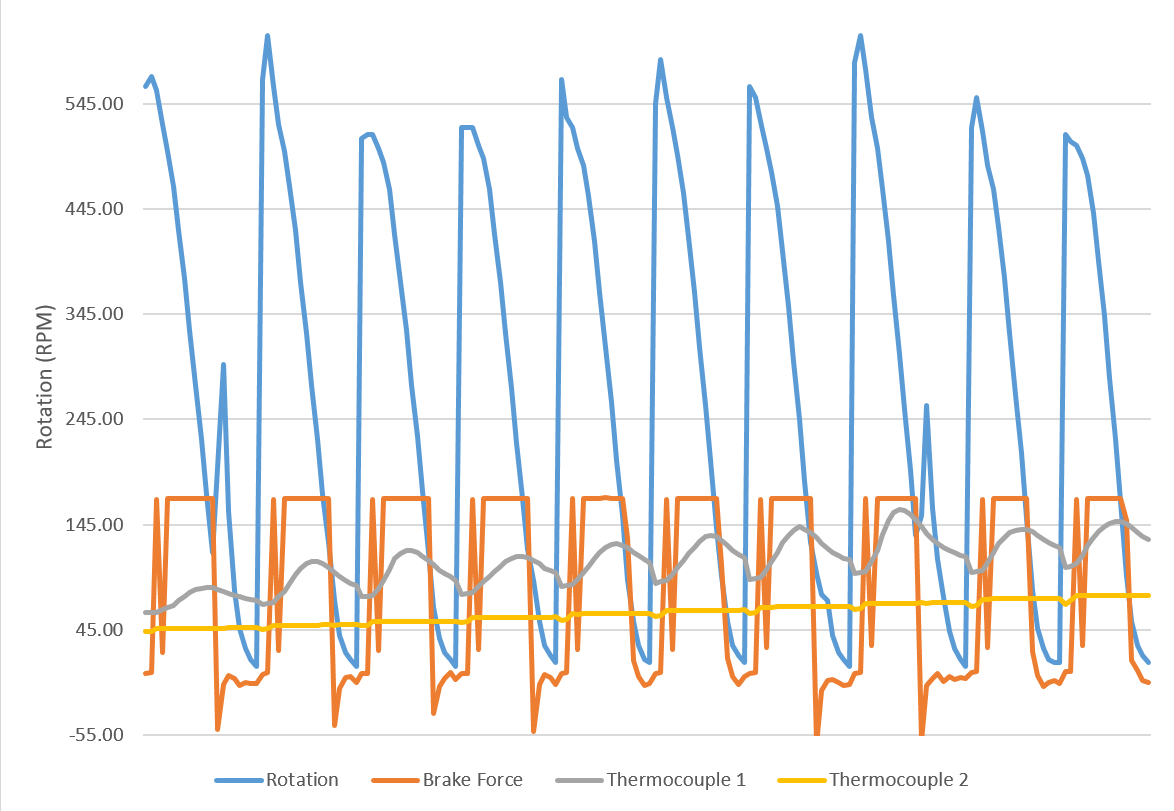
\includegraphics[width=.8\textwidth]{figuras/fig-test-first-ten-snubs}
				\caption{Measurements of the first ten snubs of the test}
				\label{fig:test-first-ten-snubs}
		\end{figure}

		On the graph from Figure \ref{fig:test-first-ten-snubs} it is possible to see the correlation between the measured quantities. Clearly the measured rotation falls rapidly as the brake force saturates to a maximum brake force value. Moreover, at each brake event, detected when the brake force increases, the temperature measured on each of thoose thermocouples bounces.
		\par

		Taking a more detailed look at the temperature variation at each snub, Figure \ref{fig:test-first-ten-snubs-force-temperature} show the measured brake force regard the measured temperature at the first ten snubs. This graph states the coorelation between the temperature of the brake pads and the braking action, and the fact that the temperature increases during the braking act is perfectly in agreement with the fact that a braking system can be analysed as a kinectic to thermal energy converter, at is was explained in Section \ref{sec:working-principles-of-disk-brake-systems}.

		\begin{figure}[htbp]
				\centering
				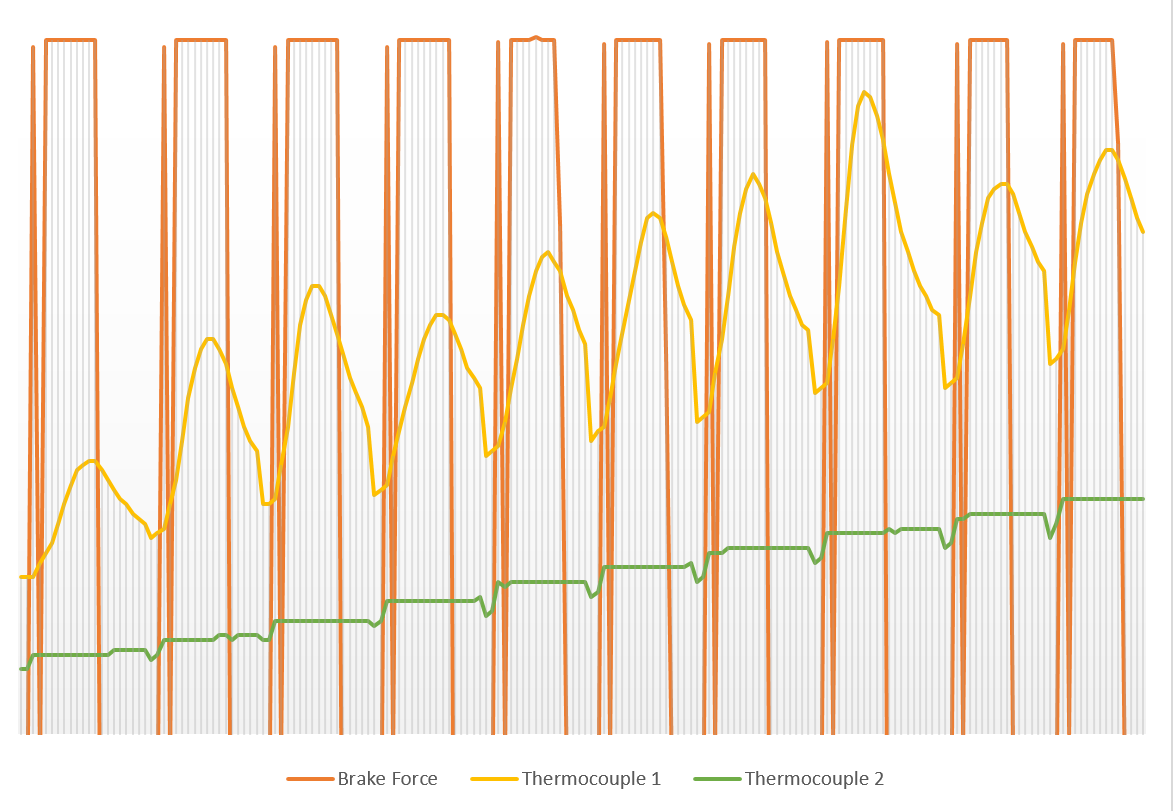
\includegraphics[width=.8\textwidth]{figuras/fig-test-first-ten-snubs-force-temperature}
				\caption{Temperature and Brake Force Measurements of The First Ten Snubs}
				\label{fig:test-first-ten-snubs-force-temperature}
		\end{figure}

		Figure \ref{fig:test-first-ten-snubs-temperature} is similar to Figure \ref{fig:test-first-ten-snubs-force-temperature}, the difference is that this time only temperature measurement is shown in order to give a sharper view of how the temperature increases during each snub.

		\begin{figure}[htbp]
				\centering
				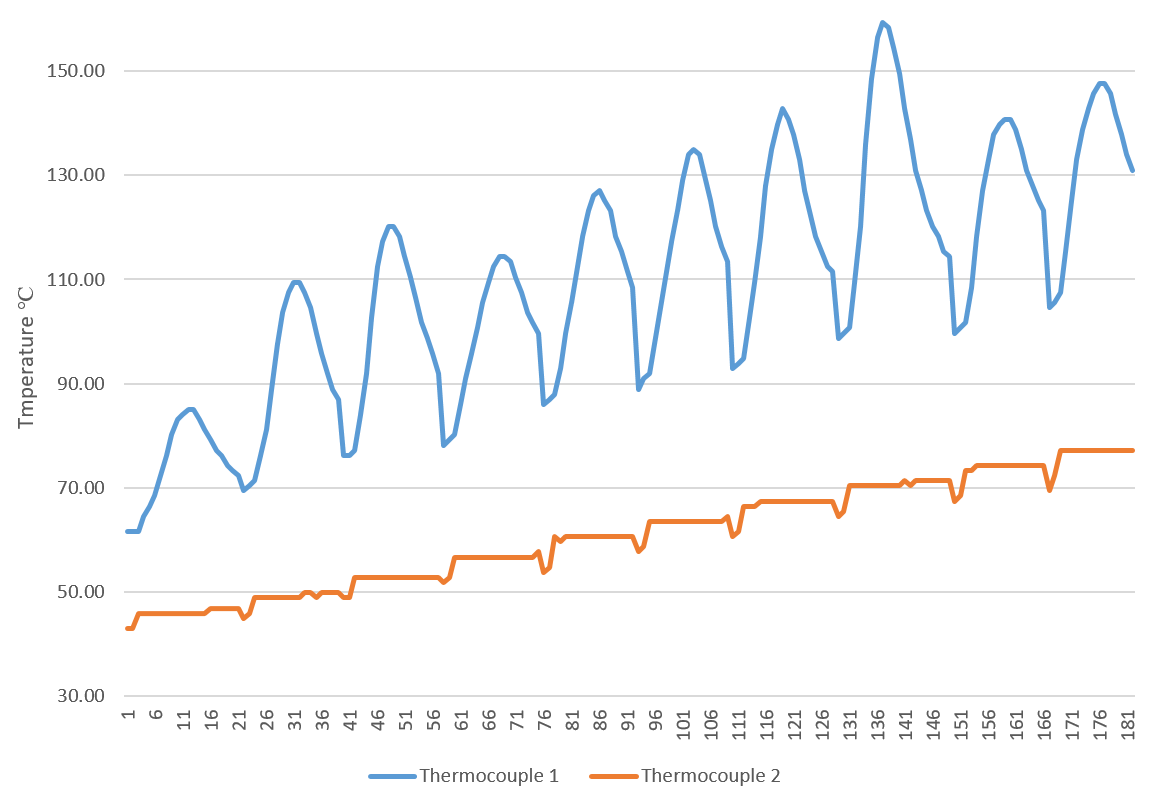
\includegraphics[width=.8\textwidth]{figuras/fig-test-first-ten-snubs-temperature}
				\caption{Temperature of The First Ten Snubs}
				\label{fig:test-first-ten-snubs-temperature}
		\end{figure}

		Figure \ref{fig:test-first-ten-snubs-force} is similar to the two previous figures, this time showing only the brake force along the first ten snubs.
		\begin{figure}[htbp]
				\centering
				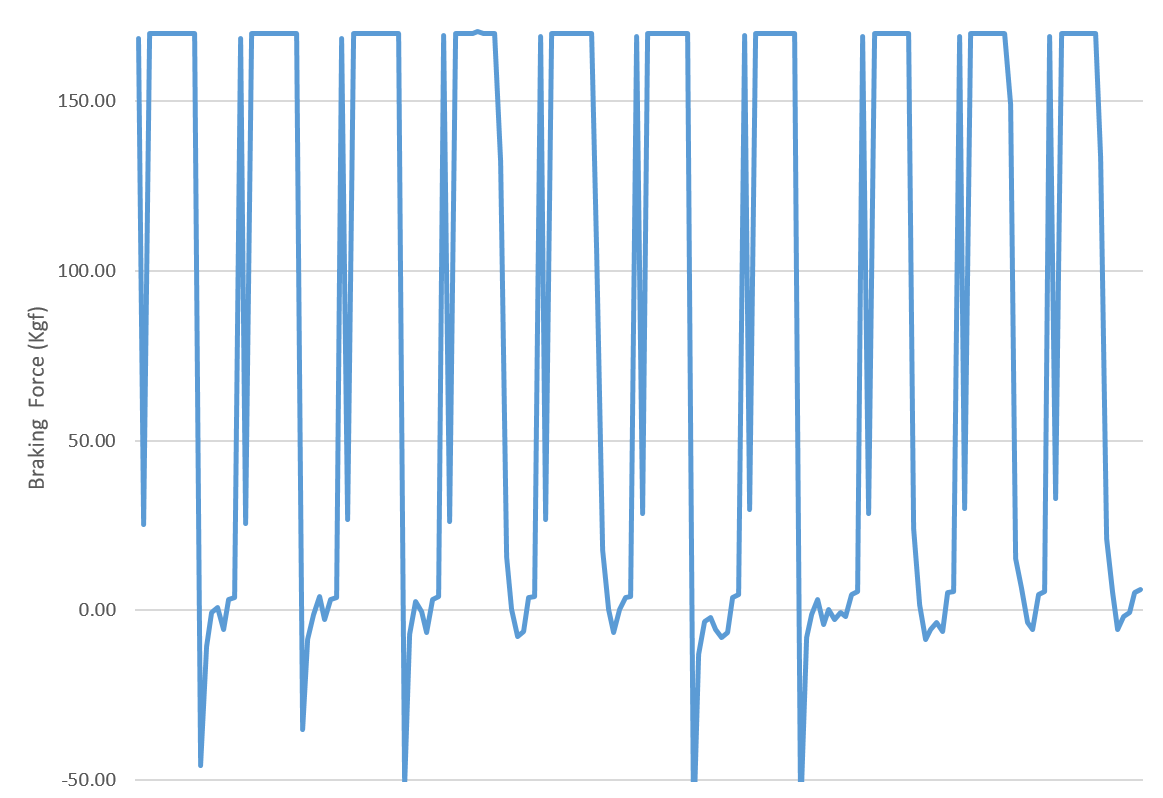
\includegraphics[width=.8\textwidth]{figuras/fig-test-first-ten-snubs-force}
				\caption{Brake Force of The First Ten Snubs}
				\label{fig:test-first-ten-snubs-force}
		\end{figure}
		\par

		Whereas the temperature increases at each snub, there may be a point where the temperature reaches a equilibrium, Figure \ref{fig:test-temperature} shows the variation of temperature during the 100 snubs, it is possible to see that even that the temperature bounces at each snub, there may be a point were the temperature stabilizes close to a certain temperature.

		\begin{figure}[htbp]
				\centering
				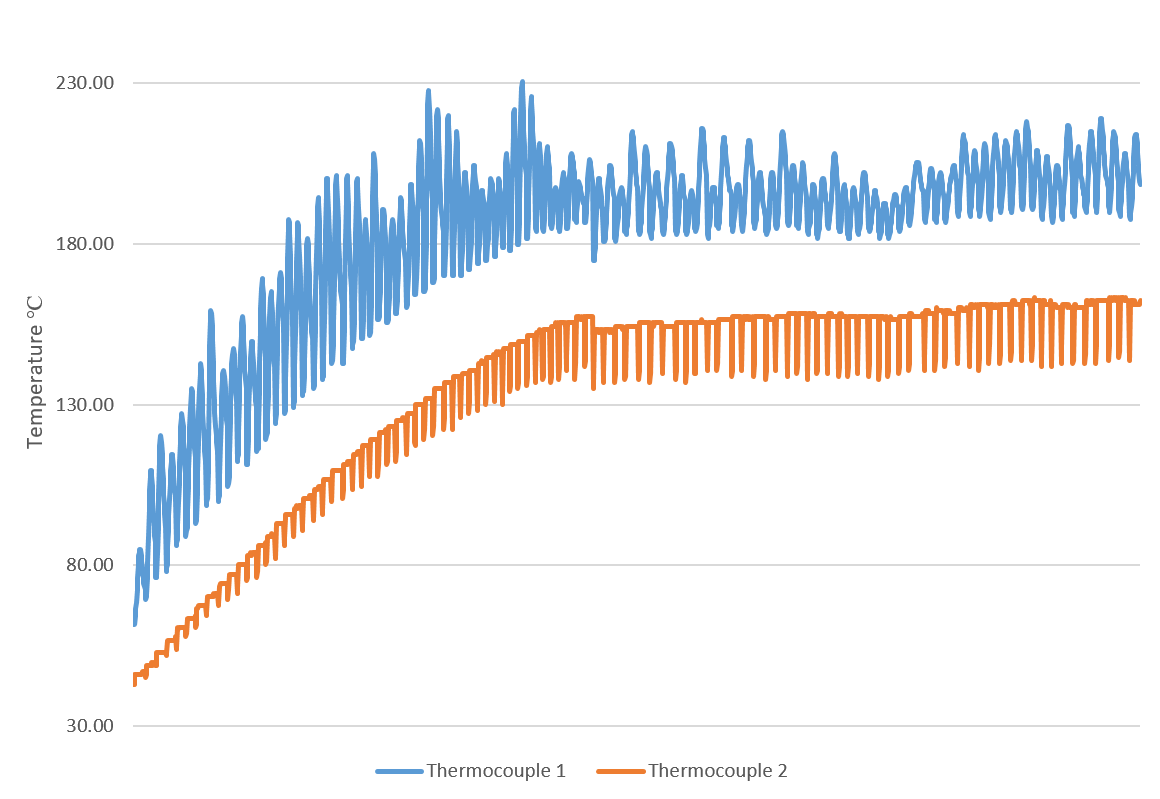
\includegraphics[width=.8\textwidth]{figuras/fig-test-temperature}
				\caption{Temperature Variation During The Whole Test}
				\label{fig:test-temperature}
		\end{figure}
		\par

		Another interisting point to analyse is the effect of the temperature of the pads and the rate of desaceleration of the rotor. Figure \ref{fig:snubs-rotation} shows the desaceleration curves at each snub and shows that during the test the brake efficiency was slightly reduced as the temperature would increase.

		\begin{figure}[htbp]
				\centering
				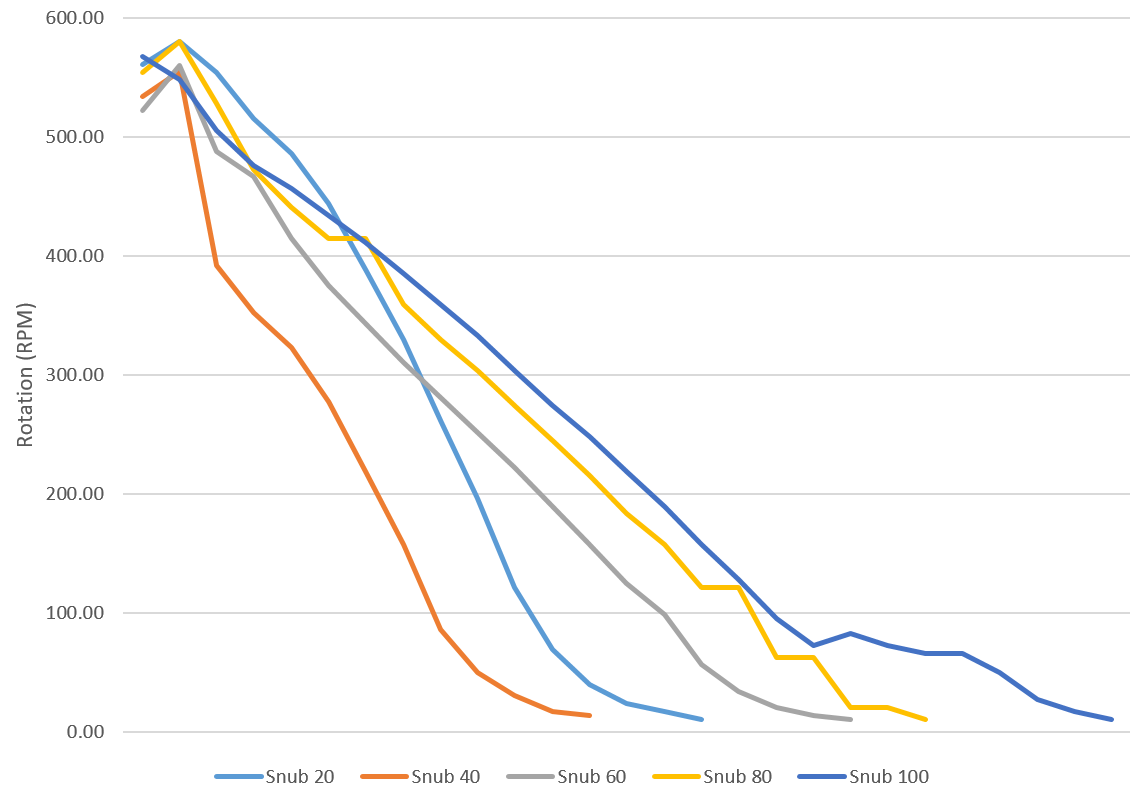
\includegraphics[width=.8\textwidth]{figuras/fig-snubs-rotation}
				\caption{Deceleration During the Whole Test}
				\label{fig:snubs-rotation}
		\end{figure}